\documentclass[14pt,a4paper]{scrartcl}
\usepackage[utf8]{inputenc}
\usepackage[english,russian]{babel}
\usepackage{indentfirst}
\usepackage{misccorr}
\usepackage{graphicx}
\usepackage{amsmath}
\usepackage{textcomp}
\usepackage{alltt}
\usepackage{amssymb}
\usepackage{pgfplots}
\graphicspath{{pictures/}}
\begin{document}
\begin{titlepage}
  \begin{center}
    \large
    МИНИСТЕРСТВО ОБРАЗОВАНИЯ И НАУКИ\\ РОССИЙСКОЙ ФЕДЕРАЦИИ
     
    \vspace{0.5cm}
 
    Федеральное государственное автономное образовательное учреждение высшего образования \\ «МОСКОВСКИЙ ФИЗИКО-ТЕХНИЧЕСКИЙ ИНСТИТУТ (научно-исследовательский институт)»
    \vspace{0.25cm}

	Физтех-школа аэрокосмических технологий
     
    Кафедра общей физики
    \vfill
     
     

    Голубятников Сергей
    \vfill
 
    \textsc{Отчёт по лабораторной работе}\\[5mm]
     
    {\LARGE Электронный парамагнитный резонанс}
  \bigskip
     
   3 курс, группа Б03-903
\end{center}
\vfill
 
\newlength{\ML}
\settowidth{\ML}{«\underline{\hspace{0.7cm}}» \underline{\hspace{2cm}}}
\hfill
\begin{minipage}{0.4\textwidth}
  Руководитель работы\\
  \underline{\hspace{\ML}} Л.\,В.~Инжечик\\
  «\underline{\hspace{0.7cm}}» \underline{\hspace{2cm}} 2021 г.
\end{minipage}%
\bigskip
 

\vfill
 
\begin{center}
  Долгопрудный, 2021 г.
\end{center}
\end{titlepage}


\tableofcontents
\addcontentsline{exp}{section}{Заголовок добавить в содержание}
\newpage


\section{Цель работы}
Исследовать электронный парамагнитный резонанс (ЭПР) в молекуле дифенилпикрилгидразила (ДФПГ). Определить $g$-фактор электрона. Измерить ширину линий ЭПР.

\section{В работе используются:}
Источник постоянного тока GPR-30H10D, 2 вольтметра GDM-8145, Фазовращатель, трасформатор ЛАТР, генератор ВЧ Г4-116, осциллограф INSTEK GDS-620, катушки, резистор.

\section{Теория}

Теория для данной лабораторной работы находится в лабораторном практикуме по общей физике Т.3. Квантовая физика на страницах \textbf{260-266}


\section{Экспериментальная установка}


Схема установки показана на рис. 1. Переменное электромагнитное поле на частоте ~100 МГц создаётся высокочастотным генератором, постоянное магнитное поле создаётся электромагнитом. Для увеличения чувствительности эксперимента образец помещают в катушку индуктивности колебательного контура. Колебательный контур состоит из катушки индуктивности и плоского конденсатора. Генератор высокой частоты не соединён с контуром непосредственно: для возбуждения колебаний в контуре служит электродинамическая связь в виде антенны, соединённой с выходом генератора. Излучаемое антенной электромагнитное поле возбуждает колебания в контуре. Для определения амплитуды этих вынужденных колебаний рядом с
катушкой индуктивности контура расположен виток приёмной катушки детектора. Колебания магнитного поля в катушке индуктивности наводят ЭДС индукции в этом витке. Детектором является высокочастотный диод. В цепь детектора подключён осциллограф.Для создания магнитного поля используется электромагнит, состоящий из пары разнесённых катушек. Ток через электромагнит контролируется по падению напряжения на резисторе,включённом в цепь питания катушек. Дополнительно к основным катушкам имеется пара
модуляционных катушек, в которые могут создавать переменное поле малой амплитуды. Для
создания переменного поля к катушкам прикладывается напряжение с трансформатора ЛАТР. Калибровка электромагнита осуществляется по измерению наводимой
ЭДС индукции в пробной катушке известной геометрии при подаче переменного тока в
соответствующие катушки электромагнита.

\begin{center}
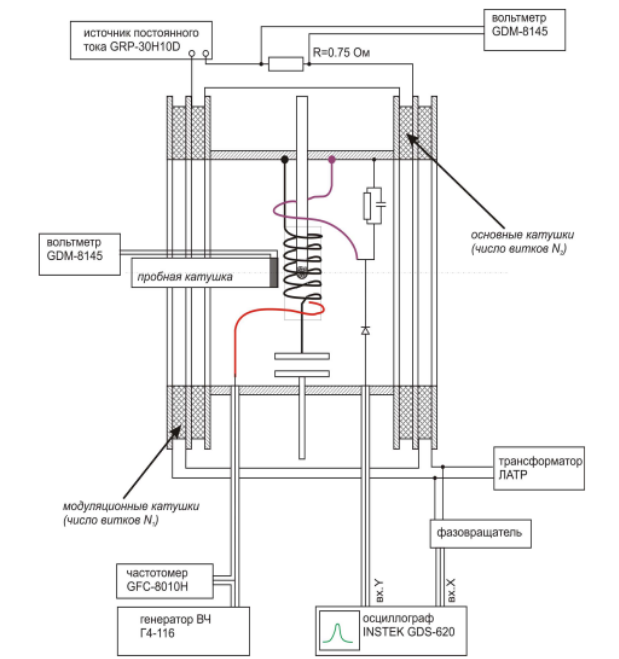
\includegraphics[scale=0.6]{Установка.png}\newline
\caption{Рис.1. Схема установки}
\end{center}


\section{Ход работы}

\subsection{Настройка ВЧ генератора}

Необходимо настроить генератор на резонансную частоту колебательного контура, определить значение частоты, определить добротность контура.

При настройке получаем:

\begin{table}[h]
    \centering
    \begin{tabular}{|c|c|c|}
    \hline
        $f_0$, МГц & $f_{+\frac{1}{2}}$, МГц & $f_{-\frac{1}{2}}$, МГц\\ \hline
        126.8 & 127.1 & 126.2 \\ \hline
    \end{tabular}
    \caption{Измерение частоты}
\end{table}

Погрешность для всех частот - цена деления шкалы 0.2МГц.\\

Определил значение добротности колебательного контура по формуле:

$$
Q_{0}=\frac{f_{0}}{f_{+\frac{1}{2}}-f_{-\frac{1}{2}}} = 120.1 \pm 20
$$

где погрешность посчитана по формуле:

$$
\sigma_{Q}=\sigma_{f} \sqrt{\left(\frac{\partial Q}{\partial f_{0}}\right)^{2}+\left(\frac{\partial Q}{\partial f_{+\frac{1}{2}}}\right)^{2}+\left(\frac{\partial Q}{\partial f_{-\frac{1}{2}}}\right)^{2}}
$$

\subsection{Наблюдение сигнала резонансного поглощения}

Необходимо пронаблюдать на экране осциллографа сигнал резонансного поглощения и зафиксировать наблюдаемую картину.

Видим, что резонансное поглощение возникает при совпадении в некоторые моменты времени поля $B(t)$ с полем резонансного поглощения на частоте колебательного контура $B_0 = \frac{hf_0}{g\mu_B}$



\subsection{Точная настройка резонансного поля и определение ширины линии}

Необходимо добиться точной настройки поля для наблюдения сигнала ЭПР, зафиксировать значение постоянного тока через основные катушки в условиях резонансного поглощения, определить ширину линии ЭПР.

Для более точной настройки и определения ширины линии резонансного поглощения удобно подать на Х-канал осциллографа напряжение, прикладываемое к модуляционным катушкам и наблюдать сигнал в XY-режиме. Фактически при этом на экране наблюдается зависимость поглощения в образце от от приложенного переменного поля.

Для определения ширины ЭПР определил по экрану осциллографа полный размах модулирующего поля $A_{\text{полн}} = 10.4 \pm 0.2$, и полную ширину кривой резонансного поглощения на полувысоте $A_{1/2} = 1 \pm 0.2$ (погрешность это размер минимального деления осциллографа). Не изменяя настроек, возьмем пробную катушку и внесем ее внутрь соленоида максимально близко к образцу. Переменное поле модуляционных катушек наводит в пробной катушке ЭДС, по которой можно определить величину поля. $\mathcal{E} = 0.97 \pm 0.04 \cdot 10^{-3}$В.

Параметры катушки: $N = 45$, $d = 15.2 \pm 0.1$. 


Вычислим амплитуду модулирующего сигнала по формуле:

$$
B_{\text {мод }}=\frac{2 \sqrt{2} \mathcal{E}}{\pi^{2} d^{2} N_{\text {проб } }  \nu} = 0.52 \pm 0.03 \text{ мТл}
$$

Погрешность: $\sigma_{B_{\text {мод }}}=\sqrt{\left(\frac{\partial B_{\text {мод }}}{\partial \mathcal{E}}\right)^{2} \sigma_{\mathcal{E}}^{2}+\left(\frac{\partial B_{\text {мод }}}{\partial d_{\text { }}}\right)^{2} \sigma_{d_{\text { } }^{2}}}$

Вычислим полуширину на высоте линии резонансного поглощения:

$$
\Delta B=\frac{A_{1 / 2}}{A_{\text {полн }}} B_{\text {мод }} = 0.116 \pm 0.012 \text{ мТл.}
$$

Погрешность: $\sigma_{\Delta B}=\sqrt{\left(\frac{\partial \Delta B}{\partial A_{\text {полн }}}\right)^{2} \sigma_{A_{\text {полн }}}^{2}+\left(\frac{\partial \Delta B}{\partial A_{1 / 2}}\right)^{2} \sigma_{A_{1 / 2}}^{2}+\left(\frac{\partial \Delta B}{\partial B_{\text {мод }}}\right)^{2} \sigma_{B_{\text {мод }}}^{2}}$

\subsection{Калибровка поля электромагнита и определение g - фактора}

Необходимо определить связь между падением напряжения на резисторе в цепи основных катушек и магнитным полем в центре магнита.


\begin{table}[h]
    \centering
    \begin{tabular}{|c|c|c|c|c|c|c|c|}
    \hline
        $V_t$, мВ & 7.5 & 9.5 & 10.8 & 11.9 & 14.3 & 16.0 \\ \hline
        $V$, мВ & 89 & 117 & 133 & 141 & 170 & 189 \\ \hline
    \end{tabular}
    \caption{Калибровочные измерения}
\end{table}

Построим график для калибровки по этим данным (рис.2):


\begin{center}
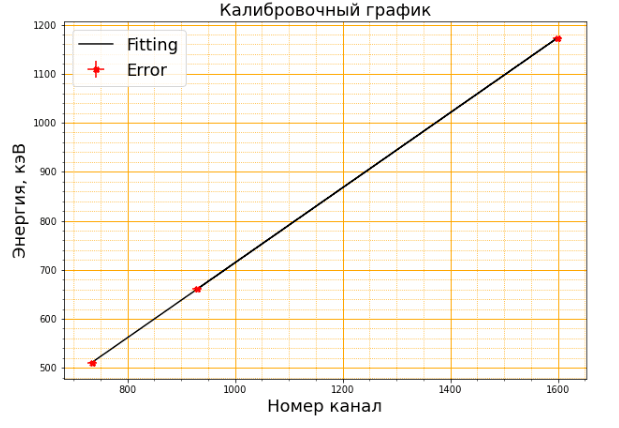
\includegraphics[scale=0.6]{calibr.png}\newline
\caption{Рис.2. График измерений для калибровки}
\end{center}



Уравнение прямой: $equation must be here$

$k = 0,134 \pm 0.009$

Погрешности согласно методу наименьших квадратов:\\


Вычислим значение индукции основного магнитного поля $B_0$ по формуле:

$$
B_{0}=\frac{4 k U}{\pi \omega d_{\text { }}^{2} N_{\text {проб }}} = 5.09 \pm 0.43 \text{ мТл}
$$

Погрешность: $\sigma_{B_{0}}=\sqrt{\left(\frac{\partial B_{0}}{\partial k}\right)^{2} \sigma_{k}^{2}+\left(\frac{\partial B_{0}}{\partial U_{R}}\right)^{2} \sigma_{U_{R}}^{2}+\left(\frac{\partial B_{0}}{\partial d_{\text { }}}\right)^{2} \sigma_{d_{\text { }}^{2}}}$\\


Теперь можем рассчитать g-фактор электрона по формуле:

$$
g=\frac{h f_{0}}{\mu_{B} B_{0}} = 1.95 \pm 0.12 
$$

Погрешность: $\sigma_{g}=\sqrt{\left(\frac{\partial g}{\partial f_{0}}\right)^{2} \sigma_{f_{0}}^{2}+\left(\frac{\partial g}{\partial B_{0}}\right)^{2} \sigma_{B_{0}}^{2}}$

Табличное значение для g-фактора электрона: $g = 2.002$. Экспериментально значение совпадает с табличным в пределах погрешности.


\section{Вывод}

В ходе лабораторной работы исследовал парамагнитный разонанс в молекуле дифенилпикрилгидразила. определил g-фактор электрона: $g = 1.9 \pm dfdf$. Также измерил ширину линий ЭПР: $\Delta B = 0.146 \pm dfs \text{ мТл.}$




\addcontentsline{toc}{section}{Список используемой литературы}

\newpage

\begin{thebibliography}{}

\bibitem{Sulsky1994}
Лабораторный практикум по общей физике: Учеб. пособие для вузов. Т. 3. Квантовая физика / Игошин Ф.Ф., Самарский Ю.А., Ципенюк Ю.М.; Под ред. Ципенюка Ю.М. - М.:Физматкнига, 2005. 432 стр.



	
\end{thebibliography}

\end{document}

